\chapter{Deus et Eliseus venerunt in mundum}
\begin{center}
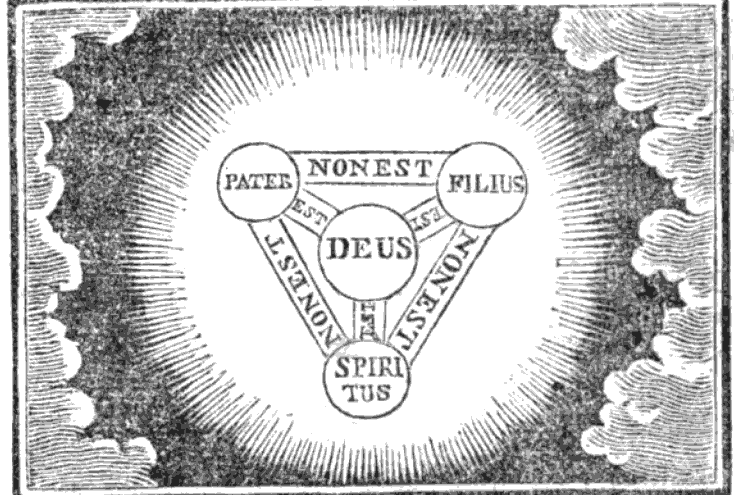
\includegraphics[scale=1.5]{God.png}
\end{center}

\section{Intended Audience}
This is intended for students who have completed Lectio 2 of Latin by the Natural Method and Chapter 3 of Lingua Latina Per Se Illustrata.

\section{Text}
Deus accepit Eliseum et ostendit Eliseo mundum. Mundus est rotundus. Mundus habet montes. Mons est altus. Altissimus Mons mundi est Mons Everest. Mundus etiam habet silvas, quae sunt magnae. Silva habet multas arbores. Arbor est alta et habet folia. Folia sunt parvae et cadunt ex arbore. In silva est umbra. Mons habet umbram. In campo non sunt multae arbores, sed paucae arbores. Mundus habet campos, qui habent foenum. Animalia, quae sunt in campo, comedunt foenum. Mons et silva et campus habent foenum. Foenum est parvus, arbor est magna. Foenum, quod est in campos, parvum est. 

Eliseus vidit in caelum. "Ecce" dixit Eliseus "Aves volant". Avis Volat per caelum. Homo est in mundo et venit per mundum. In caelo sunt nubes. Aves volant per nubes. Nubes habent umbram in mundo. Eliseus non volat, sed venit in mundo. Deus non volat, sine loco est. Iesus volavit. Deus volvait in nube ignis cum Moyse et Filiis Israel. Deus apparuit Moysen et Aaron et Filios Israel in Monte Horeb in Exodo in Nube. 

Deus etiam ostendit Eliseo Caelum. Caelum habet stellas. Stellae habent ignem in semetipis.  Moyses scripsit in Geneseo, Deus fecit in caelo luminaria. Maius luminarium regnat diem, et minora luminaria regnat noctem. Maius Eliseus fuit propheta. Minus Eliseus est filius meus parvus. In nocte sunt stellae et luna. Stellae et Luna splendent in nocte. Luna maius luminarium in nocte. Stellae minores sunt luminaria in nocte. 